\documentclass[10pt,fleqn]{article} % Default font size and left-justified equations
\usepackage[%
    pdftitle={Centrale Supelec 2018},
    pdfauthor={UPSTI}]{hyperref}

\input{style/new_style}
\input{style/macros_SII}
\usepackage{multicol}
\usepackage{siunitx}
%\usepackage{picins}
\fichetrue
%\fichefalse

\proftrue
\proffalse

%\tdtrue
\tdfalse

\courstrue
\coursfalse

% -------------------------------------
% Déclaration des titres
% -------------------------------------

\def\discipline{Sciences \\Industrielles de \\ l'Ingénieur}
\def\xxtete{Sciences Industrielles de l'Ingénieur}


\def\classe{\textsf{PSI$\star$ -- MP}}
\def\xxnumpartie{CCS 2018}
\def\xxpartie{Modéliser le comportement statique des systèmes mécaniques}

\def\xxnumchapitre{}%Révision 1 \vspace{.2cm}}
\def\xxchapitre{Concours Centrale Supelec PSI 2018}

\def\xxposongletx{2}
\def\xxposonglettext{1.45}
\def\xxposonglety{16}%16

\def\xxonglet{\textsf{Rév -- Stat}}

\def\xxactivite{TD 01}
\def\xxauteur{\textsl{UPSTI}}


\def\xxtitreexo{Tour en fosse utilisé pour le reprofilage des roues ferroviaires}
\def\xxsourceexo{\hspace{.2cm} \footnotesize{Concours Centrale Supelec PSI 2018}}

\def\xxcompetences{%
\textsl{%
%\textbf{Savoirs et compétences :}\\
}}

\def\xxfigures{
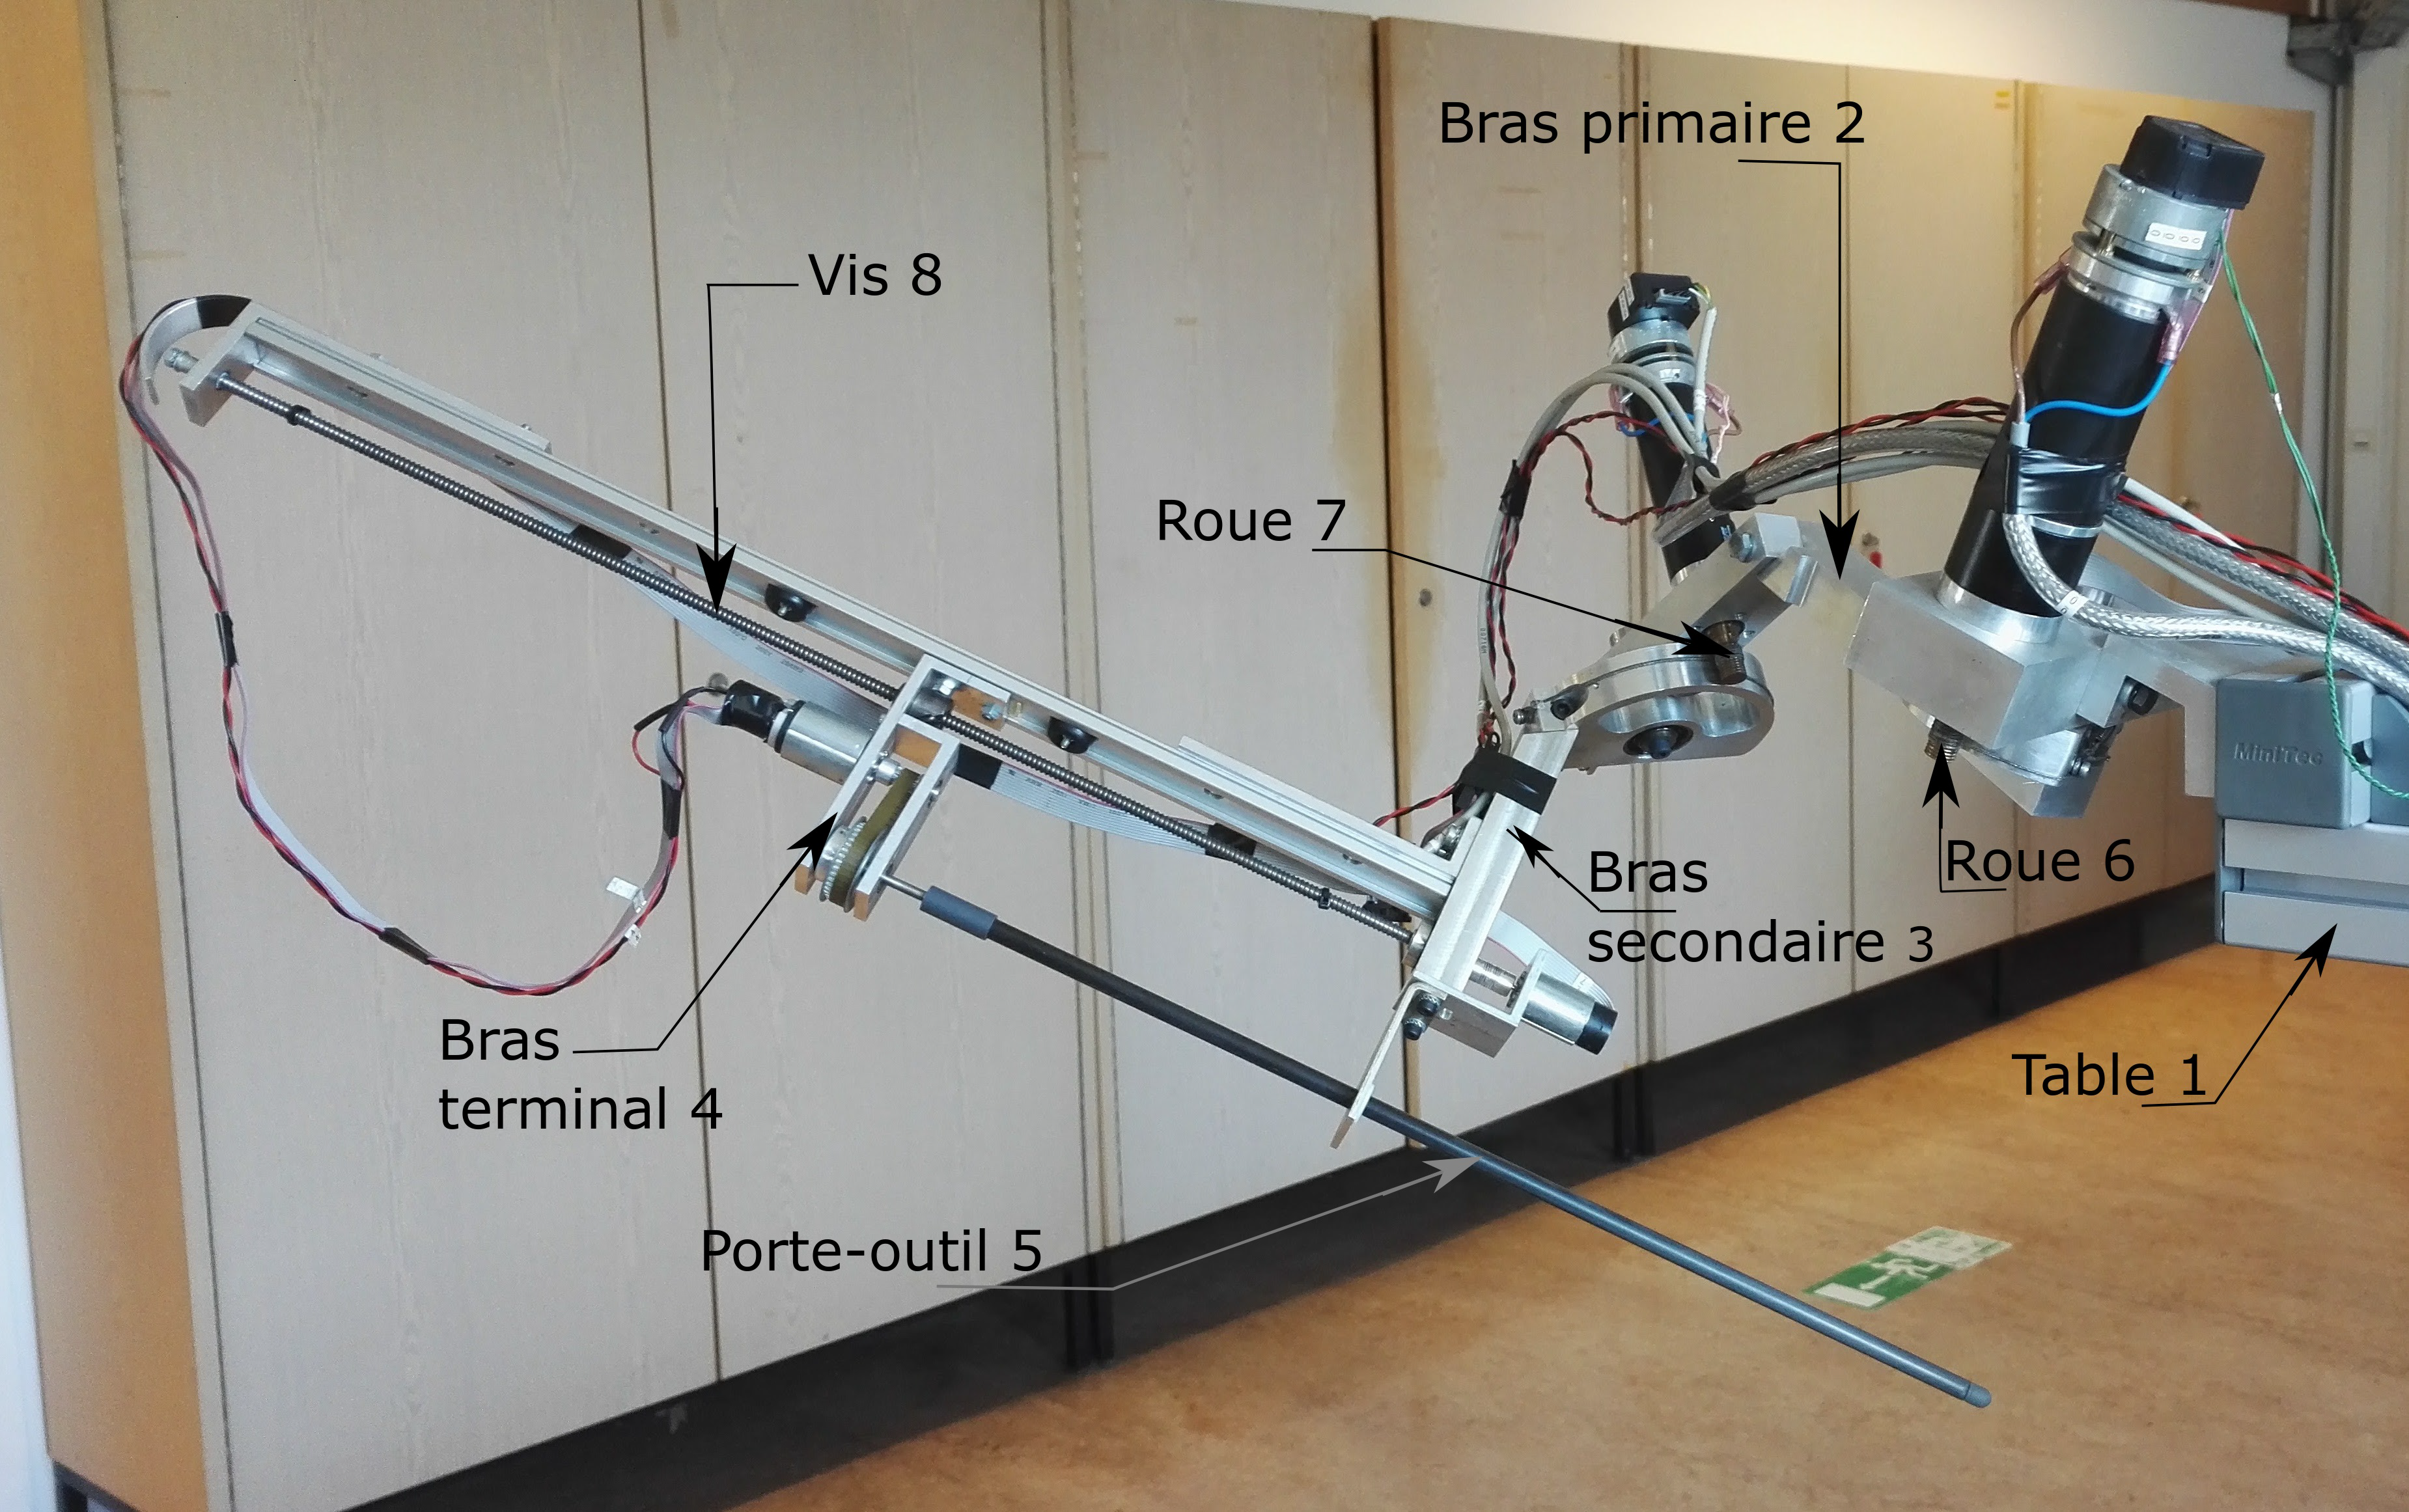
\includegraphics[width=.55\textwidth]{images/fig_00}
}%figues de la page de garde

\def\xxpied{%
Tour en fosse utilisé pour le reprofilage des roues ferroviaires\\
Concours Centrale Supelec -- PSI 2018%
}

\setcounter{secnumdepth}{5}
%---------------------------------------------------------------------------

\usepackage{bm}
\begin{document}
%\chapterimage{png/Fond_Cin}
\input{style/new_pagegarde}
\vspace{4.5cm}
\pagestyle{fancy}
\thispagestyle{plain}


\def\columnseprulecolor{\color{ocre}}
\setlength{\columnseprule}{0.4pt} 

\section{Contexte et étude préliminaire}

\begin{obj}
Valider la pertinence de l’utilisation d’une machine spéciale appelée tour en fosse pour le reprofilage
des roues ferroviaires.
\end{obj}

\subparapgraph{}

\begin{itemize}
\item Pour la méthode $a$, $t_{i1} = t_3 +t_4 = \SI{14}{h}= \SI{840}{min}.
\item Pour la méthode $b$, $t_{i2} = \left( 6\times 3 \times 2 \right)t_5 +t_6 = \SI{545}{min}.
\end{itemize}

Le gain de temps $\Delta t_i = t_{i1}-t_{i2}=\SI{295}{min}$.



\end{document}

\subparagraph{}\textit{}

\begin{center}
\includegraphics[width=\linewidth]{images/img_04}
%\textit{}
\end{center}

